\documentclass[aspectratio=169]{beamer}


\usetheme{default}
\setbeamertemplate{navigation symbols}{}
\setbeamertemplate{itemize item}{\color{black}\textbullet}
\setbeamertemplate{itemize subitem}{\color{black}\textbullet}
\usepackage{xcolor}
\definecolor{navy}{RGB}{0, 0, 128}


\begin{document}


\begin{frame}
\centering
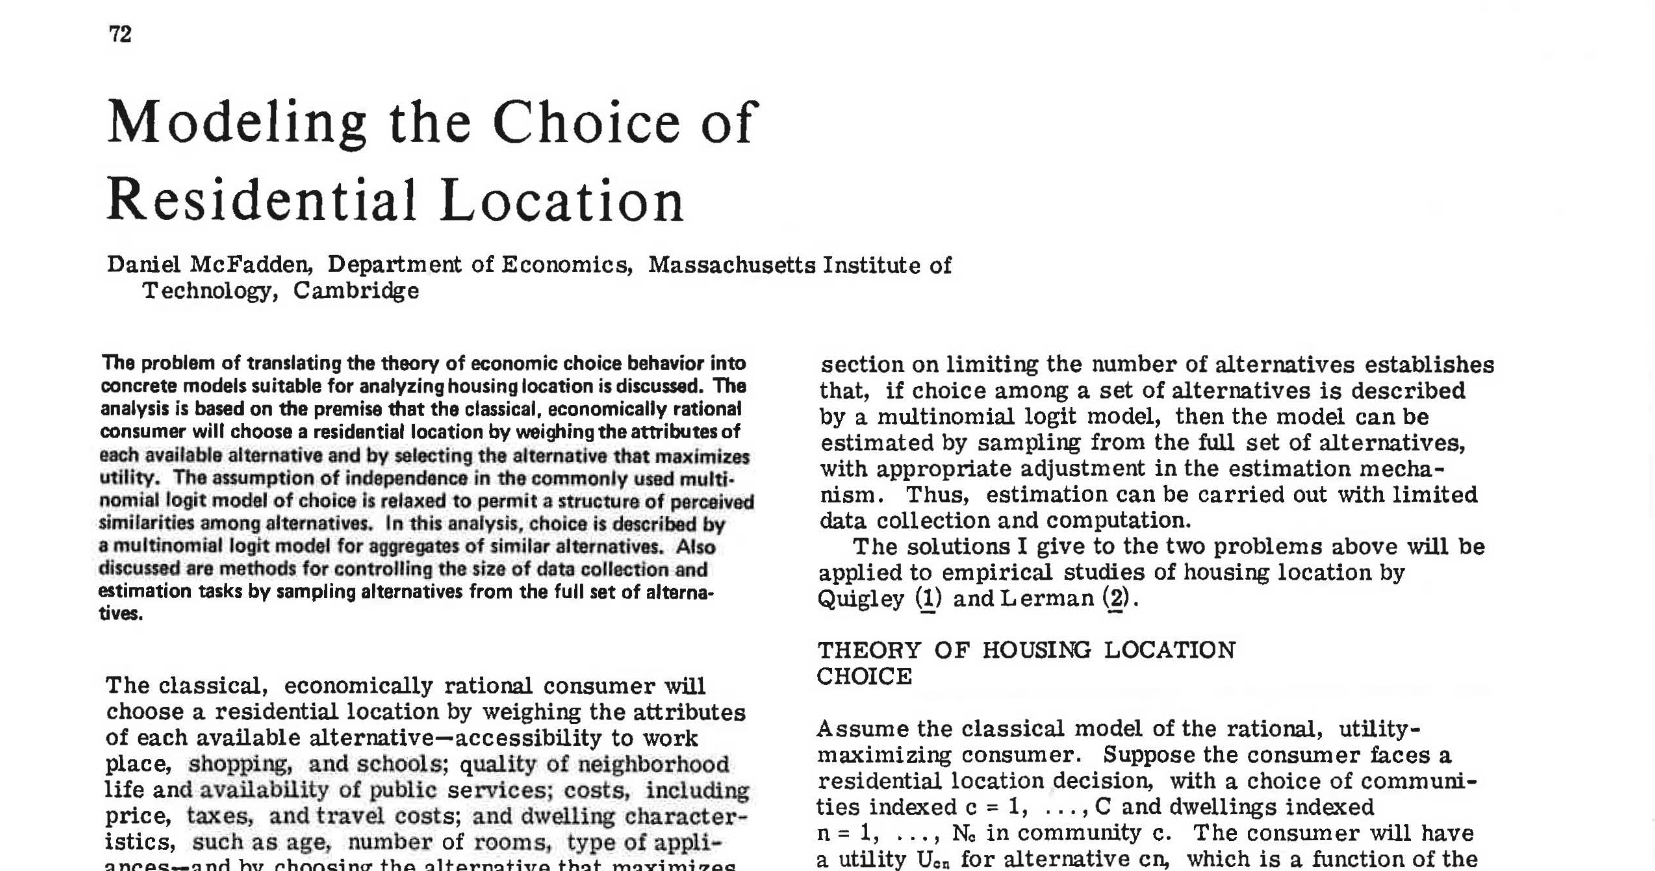
\includegraphics[width=\textwidth]{mcfadden1978cover.jpg}
\end{frame}


\begin{frame}
\centering
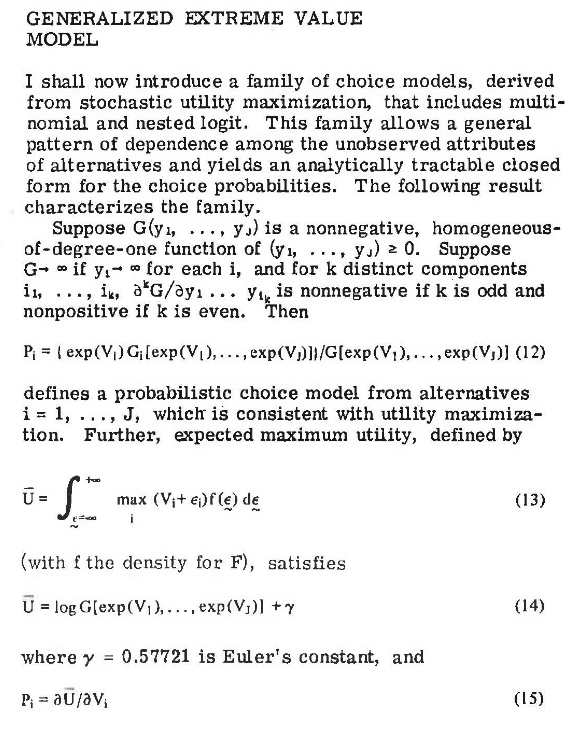
\includegraphics[width=.9\textwidth]{mcfadden1978thm1.jpg}
\end{frame}






\begin{frame}


\bigskip{}


Let $Y_{j}=\exp(u_{j})$. Consider function $G(Y_{1},\ldots,Y_{J}): \mathbb{R}^{J} \to \mathbb{R}$


\bigskip{}


\onslide<2->{
If $G$ satisfies:


\begin{itemize}
\item[]
\item $G \geq 0$
\item[]
\item Homogeneous of degree $k$
\item[]
\item $G \to \infty$ as $Y_{j} \to \infty$ for any $j$
\item[]
\item Cross partial derivatives weakly alternate in sign, beginning with $G_{i} \geq 0$
\end{itemize}
}


\end{frame}


\begin{frame}


Then:


\only<1>{
\begin{align*}
F(u_1,\ldots,u_J) = \exp[-G(Y_1,\ldots,Y_J)]
\end{align*}
}


\onslide<2->{
\begin{align*}
F(u_1,\ldots,u_J) = \exp[-G(Y_1,\ldots,Y_J)]
\end{align*}


is the CDF of a multivariate extreme value distribution
}


\bigskip{}


\onslide<3->{
And the choice probabilities are:


\begin{align*}
P_{i} = \frac{Y_{i}G_{i}}{G}
\end{align*}


where $G_i$ is the derivative of $G$ with respect to $Y_i$
}


\end{frame}


\begin{frame}


Alternative formulation:


\only<1>{
\begin{align*}
P_i = \frac{\partial \log(G)}{\partial u_i}
\end{align*}
}


\onslide<2->{
\begin{align*}
P_i = \frac{\partial \log(G)}{\partial u_i}
\end{align*}


\bigskip{}


Key insight: $\log(G)$ (plus Euler's constant) $=$ expected utility \textbf{for any GEV model}
}




\end{frame}


\begin{frame}


Multinomial Logit Case


\only<1>{
\begin{align*}
G = \sum_{j=1}^{J}\exp(u_j)
\end{align*}
}


\onslide<2->{
\begin{align*}
G = \sum_{j=1}^{J}\exp(u_j)
\end{align*}


Taking derivative of $\log(G)$:
}


\onslide<3->{
\begin{align*}
P_i &= \frac{\partial \log(G)}{\partial u_i}\\
&= \frac{\exp(u_i)}{\sum_{j=1}^{J}\exp(u_j)}
\end{align*}
}


\onslide<4->{
This gives multinomial logit probabilities
}


\end{frame}


\begin{frame}


Nested Logit Case


\bigskip{}


Two nests $(F, NF)$ and no-purchase option $N$:


\only<1->{
\begin{align*}
G &= \left(\sum_{j\in F}\exp\left(\frac{u_j}{\lambda_F}\right)\right)^{\lambda_F}+\left(\sum_{j\in NF}\exp\left(\frac{u_j}{\lambda_{NF}}\right)\right)^{\lambda_{NF}} + \exp(u_N)
\end{align*}
}


\onslide<2->{


For $k \in F$:
}


\onslide<3->{
\begin{align*}
P_k = \frac{\exp\left(\frac{u_k}{\lambda_F}\right)\left(\sum_{j\in F}\exp\left(\frac{u_j}{\lambda_F}\right)\right)^{\lambda_F-1}}{\left(\sum_{j\in F}\exp\left(\frac{u_j}{\lambda_F}\right)\right)^{\lambda_F}+\left(\sum_{j\in NF}\exp\left(\frac{u_j}{\lambda_{NF}}\right)\right)^{\lambda_{NF}}+\exp(u_N)}
\end{align*}
}


\end{frame}


\end{document}
